\section{Conclusion}
\label{sec:moe_conclusion}

In this chapter, we provide a data-driven control design that reasons about the
effects of contact forces on the hybrid system.
%
We incorporate accurate system model in the training via linear complementarity
formulation, and infer mixture of expert controllers.
%
The learning framework also provides a gating network, which selects an expert
for every observed state.
%
From simulation and real-world experiments, we demonstrate that the learned
policy leverages the advantages of contact in some states and minimizes its
adverse effects in others.
%
Moreover, the gating network is able to characterize the states prone to
contact, and selects the expert trained to react to the outcomes of potential
contacts.

\begin{figure}[H]
    \centering
    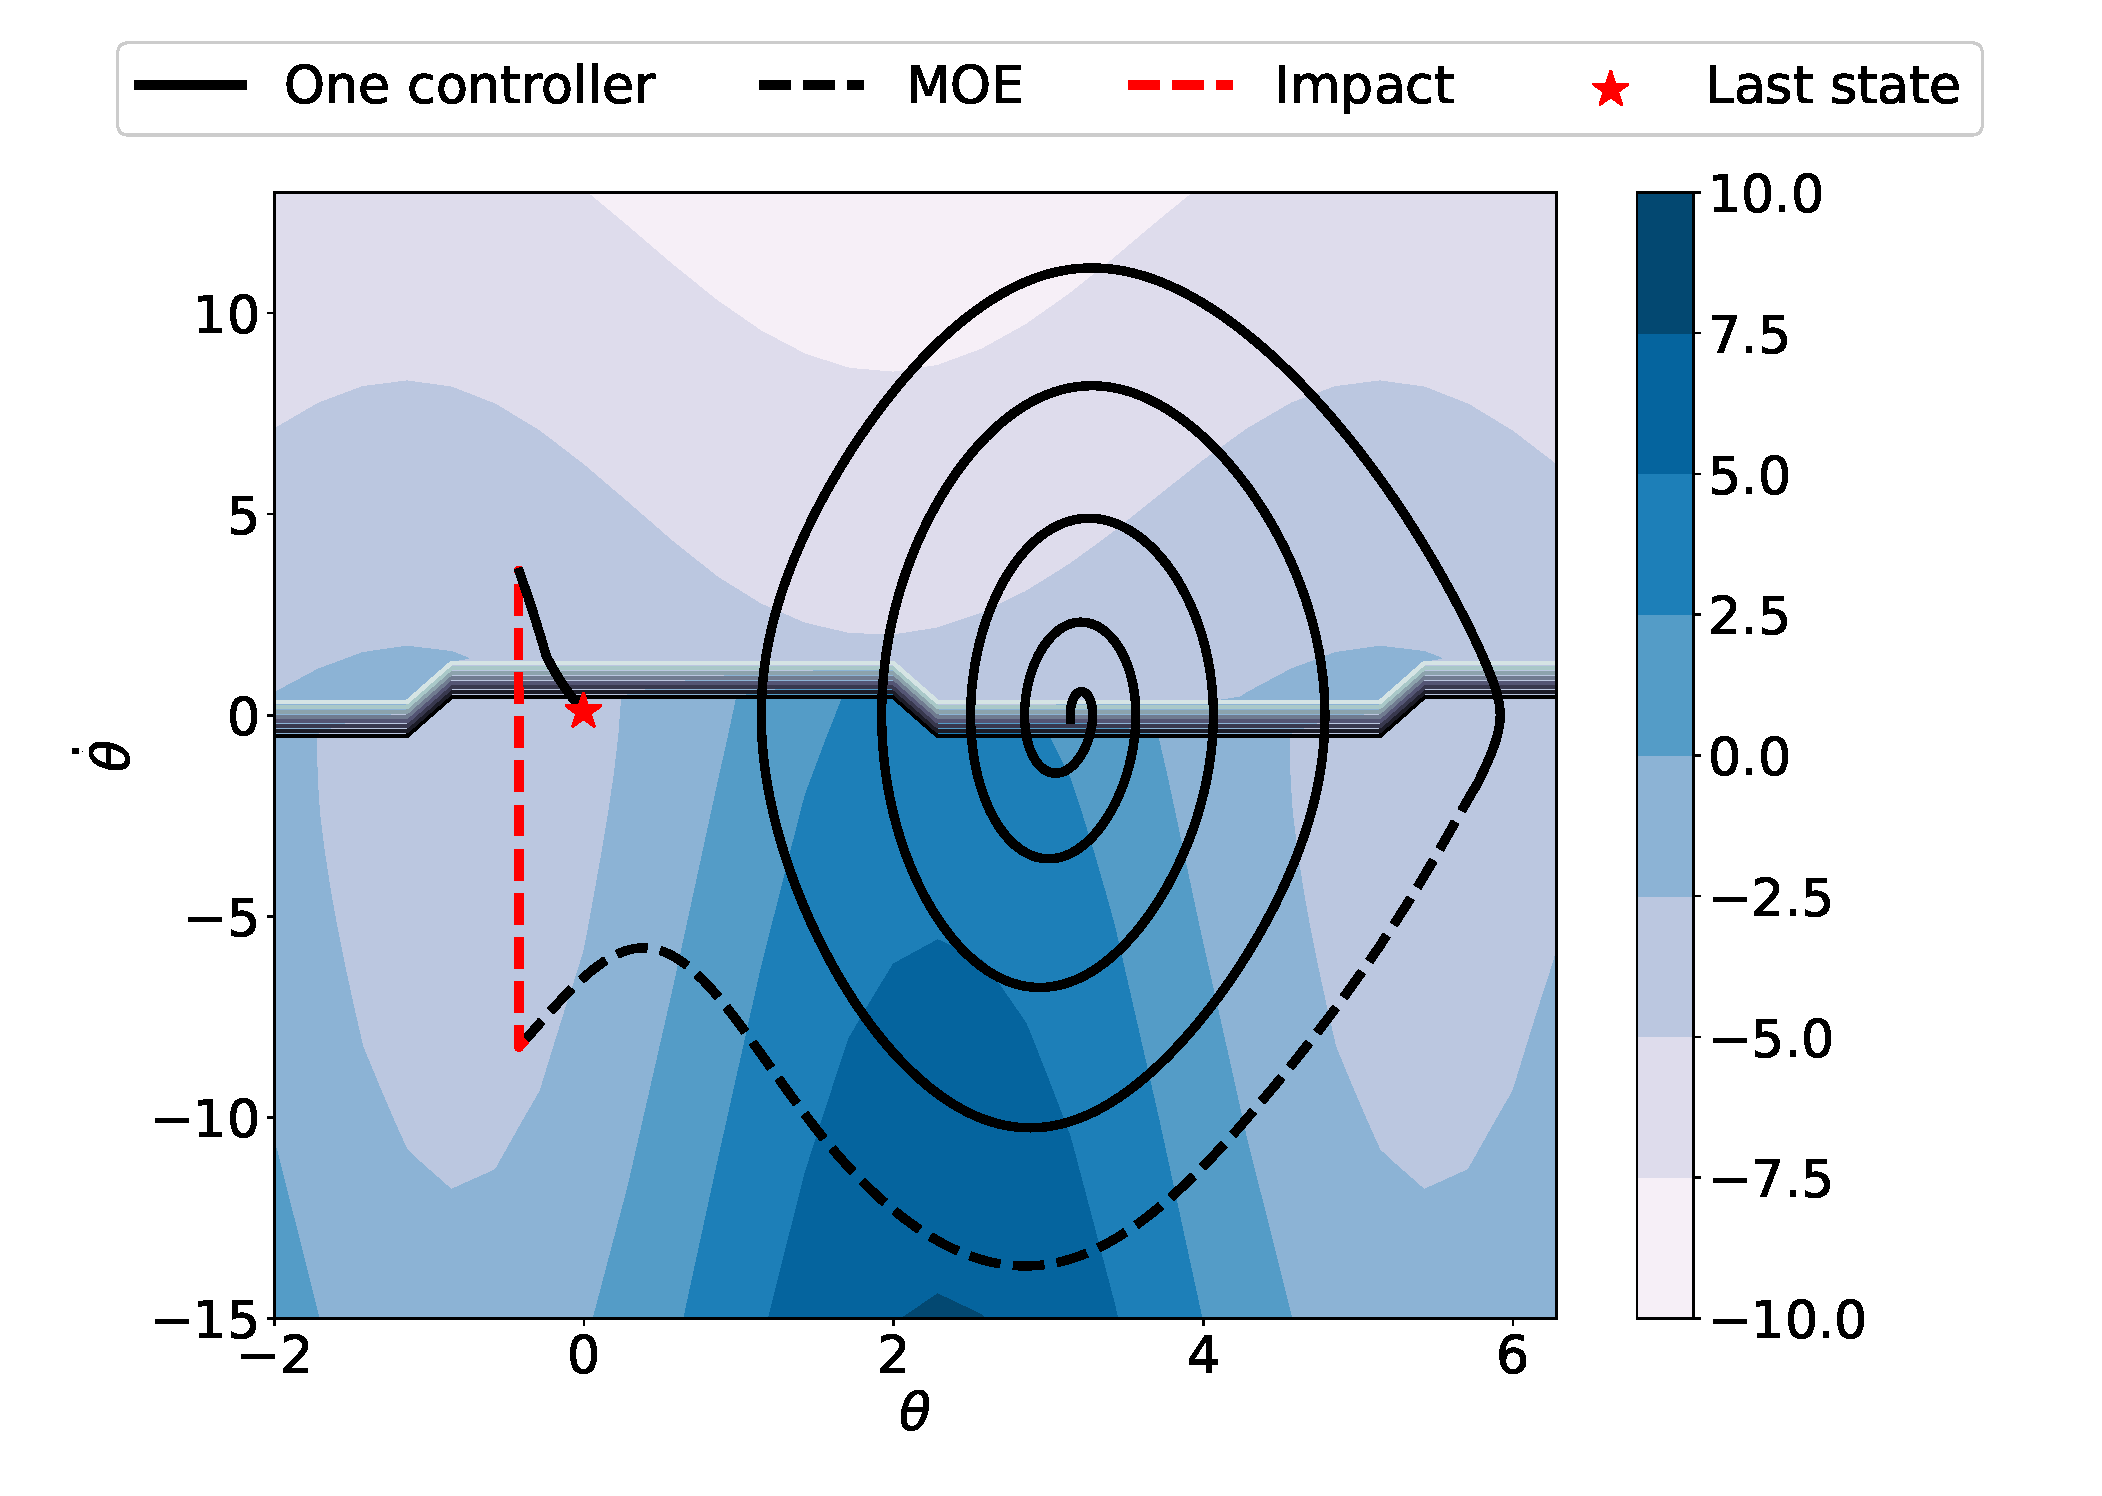
\includegraphics[width=0.7\linewidth]{contANDMOE.eps}
    \caption{The performance of the MOE controller compared to the single
    controller in Figure~\ref{fig:continuous_control}}.
    \label{fig:contandmoe}
\end{figure}